\documentclass[11pt,a4paper]{article}

% --- Packages ---
\usepackage[utf8]{inputenc}
\usepackage[T1]{fontenc}
\usepackage[margin=1in]{geometry}
\usepackage{amsmath,amssymb,amsthm}
\usepackage{hyperref}
\usepackage{xcolor}
\usepackage{graphicx}
\usepackage{enumitem}
\usepackage{booktabs}
\usepackage{tabularx}
\usepackage{fancyhdr}
\usepackage{cite}
\usepackage{float}
\usepackage{caption}
\usepackage{listings}
\usepackage{tikz}
\usetikzlibrary{arrows.meta, positioning, shapes, fit, backgrounds}

% --- Metadata ---
\title{\textbf{CRABS: Cryptographic Attribute-Based State Machines}\\[4pt]
\large \textit{A Protocol for Self-Sovereign Attribute-Based Authorization with Convergent State}}
\author{Victor J. Morrow\\[4pt]
\textit{Prometheus}\\[4pt]
\texttt{victor.j.morrow@gmail.com}}
\date{}

% --- Styling ---
\pagestyle{fancy}
\fancyhf{}
\fancyhead[L]{\small CRABS: Cryptographic Attribute-Based State Machines}
\fancyhead[R]{\small Victor J. Morrow}
\fancyfoot[C]{\thepage}
\renewcommand{\headrulewidth}{0.4pt}

\definecolor{codebg}{rgb}{0.95,0.95,0.95}
\lstset{
  basicstyle=\ttfamily\small,
  backgroundcolor=\color{codebg},
  frame=single,
  breaklines=true,
  aboveskip=8pt,
  belowskip=8pt,
  tabsize=2,
  showstringspaces=false
}

% --- Commands ---
\newcommand{\crab}{\textsc{CRABS}}
\newcommand{\abe}{\textsc{ABE}}
\newcommand{\crdt}{\textsc{CRDT}}
\newcommand{\ecdsa}{\textsc{ECDSA}}
\newcommand{\msk}{\textsc{MSK}}
\newcommand{\mpk}{\textsc{MPK}}

\begin{document}

\maketitle

\begin{center}
\rule{0.5\textwidth}{0.4pt}
\end{center}

\begin{abstract}
\noindent Attribute-Based Encryption (ABE) provides fine-grained access control by associating decryption keys with sets of attributes. However, ABE suffers from a fundamental limitation: only a central authority with the master secret key can issue or modify attributes. This creates a single point of trust, hinders self-sovereign identity, and makes dynamic attribute management impractical. We present \crab{}, a protocol that unifies ABE with Conflict-free Replicated Data Types (CRDTs) and protocol state machines. In \crab{}, \textit{attributes themselves are the state of a state machine}, and changing an attribute is a protocol-governed transition. This eliminates the central authority problem while preserving ABE's cryptographic guarantees. We describe the protocol's architecture, algorithms, security properties, and limitations, and discuss applications to decentralized organizations, resource-constrained environments, and self-sovereign identity systems.
\end{abstract}

% ======================================================================
\section{Introduction}
% ======================================================================

\subsection{The Problem}

Attribute-Based Encryption (ABE), introduced by Sahai and Waters~\cite{sahai2005fuzzy}, revolutionized cryptographic access control by allowing encryption policies to reference descriptive attributes rather than specific identities. A ciphertext encrypted under the policy \texttt{(role: manager AND department: engineering)} can be decrypted by any user holding a key with those attributes---without the encryptor knowing the recipients in advance.

Despite its power, ABE has a critical operational limitation:

\begin{quote}
\textbf{Only the authority holding the Master Secret Key (MSK) can issue, modify, or revoke attributes.}
\end{quote}

This creates several problems:

\begin{enumerate}[leftmargin=*,label={\arabic*.}]
    \item \textbf{Centralized trust}---The authority is a single point of compromise. A malicious or compromised authority can issue arbitrary attributes to any user.
    \item \textbf{Static attribute sets}---Attributes are typically issued at key generation time and are difficult to change. A user who changes departments, gets married, or is promoted must obtain an entirely new key from the authority.
    \item \textbf{No audit trail}---Attribute changes are not recorded. There is no cryptographic proof of when or why an attribute was granted or revoked.
    \item \textbf{No self-sovereignty}---Users cannot assert their own attributes (e.g., a phone number, a nickname) without going through the central authority.
    \item \textbf{Revocation is hard}---Revoking a user's attributes typically requires re-encrypting all data or maintaining complex revocation lists.
\end{enumerate}

\subsection{Our Approach}

We observe that these problems arise from treating attributes as \textit{static cryptographic material} rather than as \textit{dynamic state}. We propose a fundamental shift:

\begin{quote}
\textbf{Attributes are not keys. Attributes are state.}
\end{quote}

In \crab{}, the set of all users and their attributes is the state of a \textbf{protocol state machine}---the Attribute Machine. Changing an attribute (granting a role, verifying an identity, self-asserting a phone number) is a \textbf{state transition} governed by the same protocol rules as any other operation. The ABE keys issued to users are \textit{derived from the current state} and become invalid when the state changes.

This approach:

\begin{itemize}[leftmargin=*]
    \item Eliminates the central authority---the \textit{protocol} is the authority
    \item Provides a full audit trail of every attribute change
    \item Allows users to self-assert attributes within policy constraints
    \item Makes revocation a natural consequence of state transitions
    \item Preserves ABE's cryptographic guarantees (collusion resistance, fine-grained policies)
\end{itemize}

\subsection{Contributions}

This paper makes the following contributions:

\begin{enumerate}[leftmargin=*,label={\arabic*.}]
    \item \textbf{The \crab{} protocol}---A unified architecture combining ABE, CRDTs, and protocol state machines for self-sovereign attribute management.
    \item \textbf{The Attribute Machine}---A state machine whose state \textit{is} the attribute universe, governed by the same protocol as application-level machines.
    \item \textbf{Atomic multi-resource locking}---A composable locking primitive for operations on scarce resources, with timeout-based liveness guarantees.
    \item \textbf{Key versioning}---A mechanism for deriving ABE keys from state versions, enabling seamless attribute updates without re-encrypting data.
    \item \textbf{Dual privacy modes}---Support for both auditable (Mode A) and privacy-preserving (Mode B) operation signatures.
\end{enumerate}

% ======================================================================
\section{Related Work}
% ======================================================================

\subsection{Attribute-Based Encryption}

ABE was introduced by Sahai and Waters~\cite{sahai2005fuzzy} as ``Fuzzy Identity-Based Encryption,'' which allowed error-tolerant identity matching. Goyal et al.~\cite{goyal2006abe} formalized Key-Policy ABE (KP-ABE), where ciphertexts are tagged with attributes and user keys embed policies. Bethencourt, Sahai, and Waters~\cite{bethencourt2007cpabe} introduced Ciphertext-Policy ABE (CP-ABE), the more intuitive variant where ciphertexts embed policies and user keys carry attributes.

\textbf{Limitation:} All these schemes require a trusted authority to generate and manage keys. Multi-authority ABE~\cite{chase2007multi} and decentralized ABE~\cite{lewko2011decentralizing} distribute trust across multiple authorities, but still require each authority to manage its own attribute domain. No existing ABE scheme treats attributes as dynamic, protocol-governed state.

\subsection{Attribute-Based Signatures}

Attribute-Based Signatures (ABS), introduced by Maji et al.~\cite{maji2011abs}, allow a user to sign a message with a policy over attributes, proving that \textit{some} user with satisfying attributes endorsed the message, without revealing which user. Okamoto and Takashima~\cite{okamoto2011abs} provided efficient constructions for circuits.

\textbf{Limitation:} ABS implementations are rare and primarily exist in research libraries. Production-ready ABS libraries are not widely available. \crab{} approximates ABS using ABE-gated ECDSA signatures, achieving the same functional properties with battle-tested primitives.

\subsection{Conflict-Free Replicated Data Types (CRDTs)}

CRDTs, formalized by Shapiro et al.~\cite{shapiro2011crdt}, are data structures that can be replicated across multiple nodes and merged without conflicts. Types include G-Counters (grow-only counters), PN-Counters (positive-negative counters), OR-Sets (observed-remove sets), LWW-Registers (last-writer-wins registers), and RGA (Replicated Growable Arrays) for collaborative text editing~\cite{levien2016rga}.

\textbf{Relevance:} CRDTs provide the convergence layer for \crab{}. Operations can be applied in any order across nodes, and the state will converge to the same result. This eliminates the need for global consensus.

\subsection{Protocol State Machines and Session Types}

Protocol state machines, also known as typestate~\cite{deline2004typestate} or session types~\cite{honda1998session}, specify valid sequences of operations on a resource. The resource's current state determines which operations are permitted next. This is the foundation of \crab{}'s resource locking protocol.

\textbf{Relevance:} \crab{} extends typestate to a decentralized, CRDT-based setting where multiple participants can observe and verify protocol compliance.

\subsection{Capability-Based Security}

Capability systems~\cite{dennis1966capability} grant access based on possession of a capability token rather than identity. \crab{}'s capability vault---where ABE-encrypted ECDSA signing keys serve as capabilities---is a direct application of this principle to the attribute-based setting.

\subsection{Self-Sovereign Identity}

Self-Sovereign Identity (SSI)~\cite{allen2016ssi} is a paradigm where individuals control their own digital identities without relying on central authorities. Verifiable Credentials (VCs) and Decentralized Identifiers (DIDs) are key building blocks.

\textbf{Relevance:} \crab{}'s Attribute Machine provides a cryptographic foundation for SSI, where attributes are self-asserted or verified by peers, and all changes are recorded in an auditable transition log.

% ======================================================================
\section{The \crab{} Protocol}
% ======================================================================

\subsection{Architecture Overview}

\crab{} consists of three layers, as shown in Figure~\ref{fig:architecture}.

\begin{figure}[H]
\centering
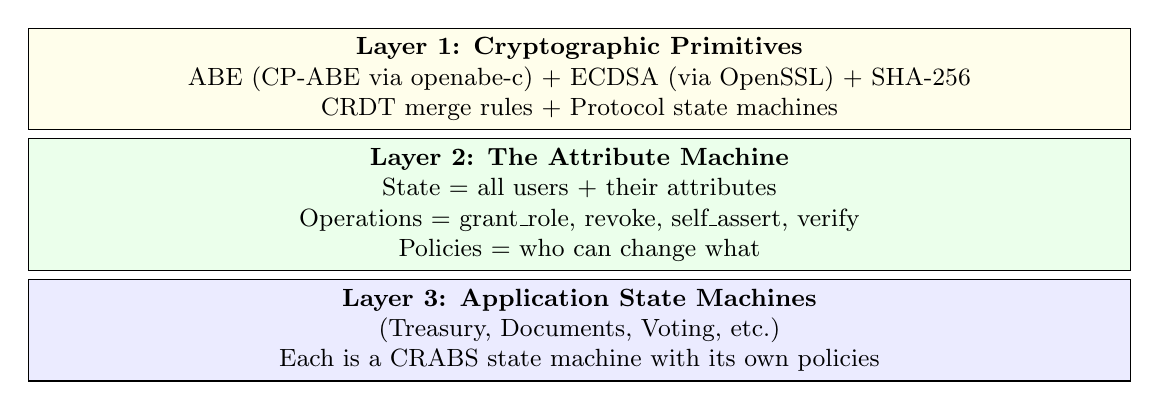
\begin{tikzpicture}[
    box/.style={draw, rectangle, minimum width=14cm, minimum height=1.2cm, align=center, font=\small},
    label/.style={font=\small\bfseries, anchor=north west}
]
    \node[box, fill=blue!8] (l3) {\textbf{Layer 3: Application State Machines}\\(Treasury, Documents, Voting, etc.)\\Each is a CRABS state machine with its own policies};
    \node[box, fill=green!8, above=0.1cm of l3] (l2) {\textbf{Layer 2: The Attribute Machine}\\State = all users + their attributes\\Operations = grant\_role, revoke, self\_assert, verify\\Policies = who can change what};
    \node[box, fill=yellow!8, above=0.1cm of l2] (l1) {\textbf{Layer 1: Cryptographic Primitives}\\ABE (CP-ABE via openabe-c) + ECDSA (via OpenSSL) + SHA-256\\CRDT merge rules + Protocol state machines};
\end{tikzpicture}
\caption{The three-layer \crab{} architecture.}
\label{fig:architecture}
\end{figure}

The Attribute Machine is the foundation. Application machines reference its state for authorization decisions. All machines follow the same protocol.

\subsection{Data Model}

The state of a \crab{} machine is a \textbf{bag of typed data items}:

\begin{lstlisting}
State = {
    items: {
        "treasury": {
            type: RESOURCE,
            crdt_type: PN_COUNTER,
            value: {ETH: 100},
            protocol_state: "idle",
            invariants: [{type: GREATER_THAN, value: 0}]
        },
        "members": {
            type: COLLECTION,
            crdt_type: OR_SET,
            value: {alice, bob, carol},
            protocol_state: "idle",
            invariants: [{type: UNIQUE}]
        },
        "seats": {
            type: RESOURCE,
            crdt_type: G_COUNTER,
            value: 50,
            protocol_state: "idle",
            invariants: [
                {type: GREATER_THAN, value: 0},
                {type: DIVISIBLE_BY, value: 2}
            ]
        }
    },
    policies: {
        "transfer": "role:admin",
        "vote": "role:member",
        "lock": "role:admin OR role:member",
        "unlock": "role:admin OR role:member"
    },
    lock_manager: { ... },
    transition_log: [...],
    version: 42
}
\end{lstlisting}

\subsection{Data Types}

\crab{} defines a small set of built-in data types, each with a CRDT merge strategy:

\vspace{4pt}
\begin{tabularx}{\textwidth}{lXcc}
\toprule
\textbf{Type} & \textbf{CRDT Strategy} & \textbf{Lock?} & \textbf{Example} \\
\midrule
\texttt{COUNTER} & G-Counter (grow-only) & No & Vote counts, reputation \\
\texttt{PN\_COUNTER} & PN-Counter (pos/neg) & For transfers & Balances, inventory \\
\texttt{SET} & OR-Set (observed-remove) & No & Member lists, permissions \\
\texttt{2P\_SET} & Two-phase set & No & Blacklists, revoked keys \\
\texttt{REGISTER} & LWW-Register (last-writer-wins) & No & Profile info, titles \\
\texttt{DOCUMENT} & RGA (replicated growable array) & No & Collaborative text \\
\texttt{RESOURCE} & PN-Counter + lock protocol & \textbf{Yes} & Treasury, seats, contracts \\
\texttt{CUSTOM} & User-defined callbacks & Configurable & Application-specific \\
\bottomrule
\end{tabularx}

\subsection{Protocol States for Resources}

Resources (items with inherent scarcity) follow a strict protocol state machine, depicted in Figure~\ref{fig:protocol}.

\begin{figure}[H]
\centering
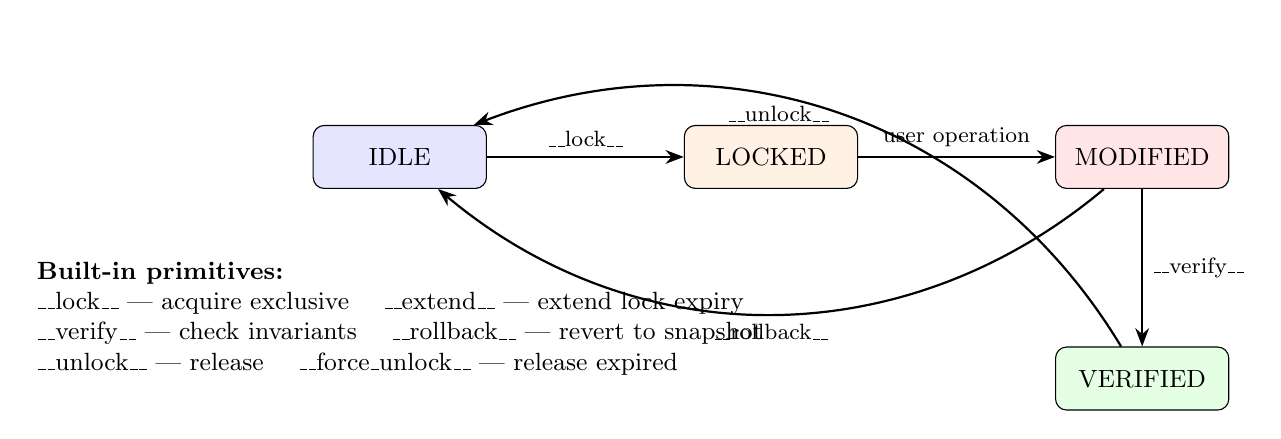
\begin{tikzpicture}[
    state/.style={draw, rectangle, rounded corners, minimum width=2.2cm, minimum height=0.8cm, align=center, font=\small},
    edge/.style={->, >=Stealth, thick, font=\footnotesize}
]
    \node[state, fill=blue!10] (idle) {IDLE};
    \node[state, fill=orange!10, right=2.5cm of idle] (locked) {LOCKED};
    \node[state, fill=red!10, right=2.5cm of locked] (modified) {MODIFIED};
    \node[state, fill=green!10, below=2cm of modified] (verified) {VERIFIED};

    \draw[edge] (idle) -- node[above] {\_\_lock\_\_} (locked);
    \draw[edge] (locked) -- node[above] {user operation} (modified);
    \draw[edge] (modified) -- node[right] {\_\_verify\_\_} (verified);

    \draw[edge, bend left=40] (modified) to node[below] {\_\_rollback\_\_} (idle);
    \draw[edge, bend right=40] (verified) to node[left] {\_\_unlock\_\_} (idle);

    % Legend
    \node[font=\small, below=0.8cm of idle, align=left, anchor=north] (legend) {
        \textbf{Built-in primitives:}\\
        \_\_lock\_\_ --- acquire exclusive \quad \_\_extend\_\_ --- extend lock expiry\\
        \_\_verify\_\_ --- check invariants \quad \_\_rollback\_\_ --- revert to snapshot\\
        \_\_unlock\_\_ --- release \quad \_\_force\_unlock\_\_ --- release expired
    };
\end{tikzpicture}
\caption{The resource protocol state machine. Resources transition through IDLE $\to$ LOCKED $\to$ MODIFIED $\to$ VERIFIED $\to$ IDLE.}
\label{fig:protocol}
\end{figure}

\subsection{The Operation}

Operations are the atomic unit of state change. They are completely generic---the state machine does not interpret operation semantics, only protocol correctness.

\begin{lstlisting}
Operation = {
    type: "transfer",                    // Arbitrary string
    payload: {amount: 10, to: "bob"},    // Application-defined

    resources: ["treasury", "seats"],    // Data items touched
    required_state: ["locked", "idle"],  // Protocol state per resource
    next_state: ["modified", "modified"],// Target state per resource

    lock_claims: [                       // Proof of lock ownership
        {resource: "treasury", token: 0xA3F7...},
        {resource: "seats",    token: 0xB7E2...}
    ],

    policy: "role:admin",                // ABE policy for authorization
    signature: 0x...,                    // ECDSA signature
    signer_id: "carol",                  // Mode A, or "" for Mode B

    lamport_time: 2042,                  // Causal ordering
    node_id: "node_7"                    // Originating node
}
\end{lstlisting}

\subsection{The Attribute Machine}

The Attribute Machine is a \crab{} state machine whose state is the set of all users and their attributes:

\begin{lstlisting}
AttributeMachine State = {
    users: {
        "alice": {
            attributes: {
                role: "writer",
                dept: "engineering",
                phone: "555-0123",          // Self-asserted
                name: "Alice Smith"         // Verified by HR
            },
            public_key: 0xABC...,
            status: "active",
            key_version: 42
        },
        "bob": { ... }
    },
    policies: {
        "grant_role":      "role:admin",
        "revoke_role":     "role:admin",
        "verify_identity": "role:admin OR role:verifier",
        "self_assert":     "role:member",
        "change_policy":   "role:admin AND weight >= 3"
    }
}
\end{lstlisting}

\textbf{Key insight:} The Attribute Machine follows the \textit{same protocol} as any other \crab{} machine. There is no privileged ``authority''---only protocol rules.

\subsection{Key Derivation and Versioning}

ABE keys are derived from the current state of the Attribute Machine:

\begin{lstlisting}
KeyEnvelope = {
    user_id: "alice",
    state_version: 42,                    // Which state version this is for
    attributes_hash: SHA256(alice_attrs), // Hash of attributes at that version
    sk_abe: ABE_keygen(MSK, "role:writer|dept:engineering|...")
}
\end{lstlisting}

Verification during any operation:

\begin{lstlisting}
function verify_key_is_current(state, key):
    if key.state_version != state.version:
        return REJECT("Key is stale. Current version: {state.version}")

    current_hash = SHA256(state.users[key.user_id].attributes)
    if key.attributes_hash != current_hash:
        return REJECT("Attributes have changed since key was issued")

    return ACCEPT
\end{lstlisting}

When attributes change, users request a key refresh:

\begin{lstlisting}
Operation: __refresh_abe_key__
Resources: [attribute_machine]
Policy: "role:member"
Effect: State machine derives new key from current attributes
        Old key is invalidated (version mismatch)
\end{lstlisting}

% ======================================================================
\section{Algorithms}
% ======================================================================

\subsection{Atomic Lock Acquisition}

\begin{lstlisting}
function atomic_acquire_locks(state, resources, lock_tokens, requester):
    acquired = []

    // Phase 1: Attempt all
    for each (resource, token) in zip(resources, lock_tokens):
        res = state.items[resource]

        if res.protocol_state != "idle":
            // Resource is locked or unavailable
            goto rollback

        if not check_policy(state, "__lock__", requester):
            goto rollback

        // Acquire
        res.protocol_state = "locked"
        res.lock_token = token
        res.lock_owner = requester
        res.lock_expiry = now() + state.config.max_lock_duration
        res.pre_lock_snapshot = snapshot(res)
        res.lock_extensions = 0
        acquired.append(resource)

    return SUCCESS

rollback:
    for each resource in acquired:
        res = state.items[resource]
        res.protocol_state = "idle"
        res.lock_token = null
        res.lock_owner = null
        res.pre_lock_snapshot = null

    return LOCK_CONTENTION
\end{lstlisting}

\textbf{Virtues:}
\begin{itemize}[leftmargin=*]
    \item Atomic---no partial lock state is ever visible
    \item Deadlock-free---all-or-nothing semantics
    \item Policy-gated---only authorized users can lock
\end{itemize}

\textbf{Limitations:}
\begin{itemize}[leftmargin=*]
    \item Requires all resources to be known in advance
    \item Contention increases with number of resources per operation
    \item No priority ordering---first-come-first-served
\end{itemize}

\subsection{Force Unlock (Timeout)}

\begin{lstlisting}
function force_unlock(state, resource, requester):
    res = state.items[resource]

    if now() < res.lock_expiry:
        return LOCK_NOT_EXPIRED

    if not state.config.allow_force_unlock:
        return FORCE_UNLOCK_DISABLED

    // Roll back to pre-lock state
    if res.pre_lock_snapshot != null:
        restore(res, res.pre_lock_snapshot)
        res.pre_lock_snapshot = null

    // Release
    res.protocol_state = "idle"
    res.lock_token = null
    res.lock_owner = null

    // Log
    log(state, {
        type: "__force_unlock__",
        resource: resource,
        forced_by: requester,
        previous_owner: res.lock_owner
    })

    return SUCCESS
\end{lstlisting}

\textbf{Virtues:}
\begin{itemize}[leftmargin=*]
    \item Guarantees liveness---no resource can be locked indefinitely
    \item Anyone can trigger---no single point of failure
    \item Rollback ensures consistency
\end{itemize}

\textbf{Limitations:}
\begin{itemize}[leftmargin=*]
    \item Rollback discards any unverified changes (by design)
    \item Requires synchronized clocks (or generous timeout margins)
    \item Malicious nodes could force-unlock immediately after expiry
\end{itemize}

\subsection{Operation Execution}

\begin{lstlisting}
function execute_operation(state, op):
    // Step 1: Prune expired locks
    prune_expired_locks(state)

    // Step 2: Verify protocol states
    for each (resource, required) in zip(op.resources, op.required_state):
        res = state.items[resource]
        if res.protocol_state != required:
            return PROTOCOL_VIOLATION

    // Step 3: Verify lock claims (for locked resources)
    for each claim in op.lock_claims:
        res = state.items[claim.resource]
        if res.protocol_state == "locked":
            if res.lock_token != claim.token:
                return LOCK_TOKEN_MISMATCH
            if res.lock_owner != op.signer_id and op.signer_id != "":
                return LOCK_OWNER_MISMATCH

    // Step 4: Verify ABE policy
    if not verify_abe_signature(state, op):
        return UNAUTHORIZED

    // Step 5: Verify key is current
    if not verify_key_is_current(state, op.signer_key):
        return KEY_STALE

    // Step 6: Execute handler (application-defined)
    result = op.handler(state, op)
    if result != SUCCESS:
        return result

    // Step 7: Transition protocol states
    for each (resource, next) in zip(op.resources, op.next_state):
        state.items[resource].protocol_state = next

    // Step 8: Log
    log(state, op)
    state.version++

    return SUCCESS
\end{lstlisting}

\textbf{Virtues:}
\begin{itemize}[leftmargin=*]
    \item All security checks happen before execution
    \item Protocol state transitions are atomic with execution
    \item Full audit trail
\end{itemize}

\textbf{Limitations:}
\begin{itemize}[leftmargin=*]
    \item Sequential within a single node (though CRDT merge allows parallel across nodes)
    \item Handler is application-defined---cannot verify its correctness cryptographically
\end{itemize}

\subsection{CRDT Merge}

\begin{lstlisting}
function crdt_merge(state_a, state_b):
    merged = copy(state_a)

    for each (name, item_b) in state_b.items:
        if name not in merged.items:
            merged.items[name] = item_b
        else:
            item_a = merged.items[name]

            switch item_a.crdt_type:
                case G_COUNTER:
                    merged.items[name].value = max(item_a.value, item_b.value)

                case PN_COUNTER:
                    merged.items[name].value.pos =
                        max(item_a.value.pos, item_b.value.pos)
                    merged.items[name].value.neg =
                        max(item_a.value.neg, item_b.value.neg)

                case OR_SET:
                    merged.items[name].value =
                        union(item_a.value, item_b.value)
                    merged.items[name].tombstones =
                        union(item_a.tombstones, item_b.tombstones)

                case LWW_REGISTER:
                    if item_b.timestamp > item_a.timestamp:
                        merged.items[name].value = item_b.value
                        merged.items[name].timestamp = item_b.timestamp

                case RGA:
                    merged.items[name].value =
                        rga_merge(item_a.value, item_b.value)

    // Merge transition logs
    merged.log = merge_sorted_logs(state_a.log, state_b.log)
    merged.version = max(state_a.version, state_b.version)

    return merged
\end{lstlisting}

\textbf{Virtues:}
\begin{itemize}[leftmargin=*]
    \item Eventual consistency without consensus
    \item Deterministic---all nodes converge to the same state
    \item Handles concurrent operations gracefully
\end{itemize}

\textbf{Limitations:}
\begin{itemize}[leftmargin=*]
    \item CRDTs have limited expressiveness (no arbitrary computation)
    \item Tombstones in OR-Sets grow unboundedly (can be garbage-collected with coordination)
    \item Last-writer-wins registers lose concurrent updates
\end{itemize}

\subsection{Key Refresh}

\begin{lstlisting}
function refresh_abe_key(state, msk, mpk, user_id, requester):
    user = state.users[user_id]

    // Verify requester is the user or an admin
    if requester != user_id
       and not check_policy(state, "refresh_key", requester):
        return UNAUTHORIZED

    // Build attribute string from current state
    attrs = []
    for each (name, value) in user.attributes:
        attrs.append("{name}:{value}")
    attr_string = join(attrs, "|")

    // Generate new key
    sk_abe = ABE_keygen(msk, mpk, attr_string)

    // Create key envelope with current state version
    envelope = {
        user_id: user_id,
        state_version: state.version,
        attributes_hash: SHA256(user.attributes),
        sk_abe: sk_abe
    }

    // Update user's key version
    user.key_version = state.version

    return envelope
\end{lstlisting}

\textbf{Virtues:}
\begin{itemize}[leftmargin=*]
    \item Keys are always derived from current state
    \item Old keys are automatically invalidated (version mismatch)
    \item No need to re-encrypt existing data---only new operations check key freshness
\end{itemize}

\textbf{Limitations:}
\begin{itemize}[leftmargin=*]
    \item Requires users to proactively refresh keys after attribute changes
    \item Brief window where old key could be used if state version check is delayed
    \item Key refresh is an online operation (requires communication with a node)
\end{itemize}

% ======================================================================
\section{Security Analysis}
% ======================================================================

\subsection{Threat Model}

We assume the following adversary capabilities:

\begin{itemize}[leftmargin=*]
    \item \textbf{Network adversary:} Can observe, delay, reorder, and drop messages
    \item \textbf{Byzantine nodes:} Up to $f$ nodes may behave arbitrarily (but not collude with the ABE authority, which is the protocol itself)
    \item \textbf{Compromised users:} Can attempt to use stale keys, forge signatures, or collude
\end{itemize}

We do \textbf{not} defend against:

\begin{itemize}[leftmargin=*]
    \item Compromise of the MSK (though the MSK can be rotated via protocol transition)
    \item Quantum attacks on bilinear pairings (post-quantum variants are future work)
    \item Sybil attacks on node identity (requires external PKI or proof-of-work)
\end{itemize}

\subsection{Security Properties}

\vspace{4pt}
\begin{tabularx}{\textwidth}{l>{\hsize=0.9\hsize}X>{\hsize=1.1\hsize}X}
\toprule
\textbf{Property} & \textbf{Mechanism} & \textbf{Guarantee} \\
\midrule
Authorization & ABE policy verification & Only users with matching attributes can perform operations \\
Authentication & ECDSA signatures & Operations are cryptographically bound to a specific key \\
Non-repudiation & Signed log entries & Past operations cannot be denied \\
Collusion resistance & ABE key randomization & Two users cannot combine keys to gain unauthorized access \\
Replay protection & Lamport clocks + nonces & Old messages cannot be replayed \\
Liveness & Lock timeout + force-unlock & No resource can be locked indefinitely \\
Confidentiality & ABE encryption & Only authorized users can decrypt operation payloads \\
Privacy (Mode B) & Optional signer omission & Verifier learns only that \textit{some} authorized user signed \\
Auditability (Mode A) & Signer identity included & Every operation is attributable to a specific user \\
\bottomrule
\end{tabularx}

\subsection{Key Compromise}

If a user's ECDSA signing key is compromised:

\begin{enumerate}[leftmargin=*,label={\arabic*.}]
    \item The user reports the compromise via a signed operation
    \item An admin revokes the user's key via a state transition
    \item The user is issued a new key pair
    \item The old key is added to a revocation set (2P-Set)
    \item Any operation signed with the old key is rejected
\end{enumerate}

If the MSK is compromised:

\begin{enumerate}[leftmargin=*,label={\arabic*.}]
    \item The MSK is rotated via a protocol transition (requires threshold of admins)
    \item All users refresh their ABE keys
    \item Old ciphertexts remain secure (the old MSK is discarded, not exposed)
    \item New ciphertexts use the new MPK
\end{enumerate}

% ======================================================================
\section{Use Cases}
% ======================================================================

\subsection{Decentralized Autonomous Organizations (DAOs)}

\crab{} provides a natural foundation for DAOs where membership is defined by attributes rather than token holdings:

\begin{lstlisting}
DAO State = {
    treasury: RESOURCE(PN_COUNTER, {ETH: 1000}),
    members: SET(OR_SET, {alice, bob, carol}),
    proposals: CUSTOM(...),
    policies: {
        "create_proposal":  "role:member",
        "vote":             "role:member",
        "execute":   "role:admin OR (votes >= 3 AND role:member)",
        "add_member":       "role:admin",
        "remove_member":    "role:admin AND weight >= 2",
        "spend_funds":      "role:admin AND weight >= 3"
    }
}
\end{lstlisting}

\textbf{Advantages over token-based DAOs:}
\begin{itemize}[leftmargin=*]
    \item Plutocracy is avoided---one member, one vote
    \item Roles enable fine-grained permissions
    \item No gas costs for voting
    \item Privacy-preserving voting (Mode B)
\end{itemize}

\subsection{Collaborative Document Review}

A document review workflow with dynamic policy updates:

\begin{lstlisting}
Document State = {
    content: DOCUMENT(RGA, "..."),
    status: REGISTER(LWW, "draft"),
    policies: {
        "edit":     "role:author",    // Only author can edit
        "submit":   "role:author",    // Author submits for review
        "review":   "role:reviewer",  // Reviewer reviews
        "approve":  "role:editor",    // Editor approves
        "publish":  "role:admin"      // Admin publishes
    }
}

// Transition: submit for review
// Effect: status -> "in_review"
//         policies.edit -> "role:reviewer"
//         policies.request_changes -> "role:reviewer"
\end{lstlisting}

\subsection{Self-Sovereign Identity}

The Attribute Machine enables a fully self-sovereign identity system:

\begin{lstlisting}
AttributeMachine State = {
    users: {
        "alice": {
            attributes: {
                // Self-asserted (any member can add)
                "nickname": "Ali",
                "phone": "555-0123",

                // Verified (requires role:verifier)
                "name": "Alice Smith (verified by HR)",
                "passport": "hash:0x... (verified by KYC)"
            }
        }
    },
    policies: {
        "self_assert":     "role:member",
        "verify":          "role:verifier",
        "revoke_claim":    "role:admin OR self"
    }
}
\end{lstlisting}

Users control their own attributes while relying on verifiers for high-assurance claims. All changes are logged and auditable.

\subsection{Supply Chain Management}

Each shipment is a resource with a protocol:

\begin{lstlisting}
Shipment Protocol:
  IDLE -> __lock__ -> LOCKED -> inspect -> MODIFIED
      -> __verify__ -> VERIFIED -> __unlock__ -> IDLE
  IDLE -> __lock__ -> LOCKED -> transfer -> MODIFIED
      -> __verify__ -> VERIFIED -> __unlock__ -> IDLE
  MODIFIED -> __rollback__ -> IDLE (if inspection fails)

Policies:
  "inspect":  "role:inspector AND org:customs"
  "transfer": "role:logistics AND org:carrier"
  "lock":     "role:inspector OR role:logistics"
\end{lstlisting}

Different organizations (customs, carriers, warehouses) have different roles, and the protocol ensures that custody transfers are atomic and auditable.

% ======================================================================
\section{Limitations}
% ======================================================================

\subsection{Cryptographic Limitations}

\vspace{4pt}
\begin{tabularx}{\textwidth}{l>{\hsize=0.8\hsize}X>{\hsize=1.2\hsize}X}
\toprule
\textbf{Limitation} & \textbf{Impact} & \textbf{Mitigation} \\
\midrule
MSK is a single point of compromise & If MSK leaks, attacker can forge any attribute & Threshold MSK schemes (future work) \\
Pairing operations are expensive & ABE operations are 10--100$\times$ slower than AES & Use ABE only for policy enforcement, not bulk encryption \\
Key size grows with attributes & Each attribute adds a group element & Limit attributes to $\sim$50 per user in practice \\
No post-quantum security & Bilinear pairings vulnerable to Shor's algorithm & Lattice-based ABE variants exist but are immature \\
\bottomrule
\end{tabularx}

\subsection{Protocol Limitations}

\vspace{4pt}
\begin{tabularx}{\textwidth}{l>{\hsize=0.8\hsize}X>{\hsize=1.2\hsize}X}
\toprule
\textbf{Limitation} & \textbf{Impact} & \textbf{Mitigation} \\
\midrule
No global consensus & State may diverge temporarily & CRDT merge guarantees eventual convergence \\
Lock contention & Multiple users competing for same resource & Short lock durations, exponential backoff \\
Tombstone growth & OR-Set tombstones grow unboundedly & Periodic garbage collection with coordination \\
Clock synchronization & Lock expiry depends on clocks & Use generous timeouts (2$\times$ network latency) \\
Online key refresh & Users must contact a node after attribute change & Can be batched or made asynchronous \\
\bottomrule
\end{tabularx}

\subsection{Expressiveness Limitations}

\vspace{4pt}
\begin{tabularx}{\textwidth}{l>{\hsize=0.8\hsize}X>{\hsize=1.2\hsize}X}
\toprule
\textbf{Limitation} & \textbf{Impact} & \textbf{Mitigation} \\
\midrule
No Turing-complete computation & Cannot express arbitrary smart contracts & \crab{} is declarative by design---policies are simpler and auditable \\
CRDTs limit data types & Not all data structures have CRDT equivalents & Custom types with user-defined merge functions \\
No automatic execution & Transitions require user action & Can be combined with cron-like schedulers \\
\bottomrule
\end{tabularx}

% ======================================================================
\section{Future Work}
% ======================================================================

\subsection{Threshold MSK}

The Master Secret Key remains a single point of compromise. A threshold scheme where the MSK is split across $n$ nodes, requiring $k$ to sign, would eliminate this vulnerability. This would make the Attribute Machine truly decentralized.

\subsection{Post-Quantum \crab{}}

Lattice-based ABE schemes are an active research area. Porting \crab{} to lattice assumptions would provide post-quantum security. The protocol architecture is agnostic to the underlying cryptographic primitives.

\subsection{Hierarchical Attribute Machines}

An organization might have multiple Attribute Machines (one per department) with cross-machine trust relationships. A machine in engineering might trust a machine in HR for \texttt{name} attributes but not for \texttt{role} attributes.

\subsection{Garbage Collection for CRDT Tombstones}

OR-Set tombstones grow unboundedly. A garbage collection protocol that safely removes tombstones after all nodes have observed the removal would be valuable for long-running state machines.

\subsection{Lightweight Clients}

The current design assumes clients can perform ABE operations. Lightweight clients (mobile, IoT) might delegate ABE operations to a trusted proxy while retaining ECDSA signing locally.

\subsection{Formal Verification}

The \crab{} protocol's safety properties (no invalid state transitions, invariant preservation, CRDT convergence) could be formally verified using a proof assistant such as Coq or Isabelle/HOL.

\subsection{Interoperability with Existing ABE Systems}

A bridge between \crab{} and existing ABE deployments would allow gradual migration. Ciphertexts encrypted under a traditional ABE authority could be re-encrypted under \crab{} policies.

\subsection{Economic Incentives for Force-Unlock}

Force-unlock is a public good---anyone can do it, but no one is incentivized to. A small reward (taken from the lock holder's stake) for force-unlocking expired locks would ensure liveness in practice.

% ======================================================================
\section{Conclusion}
% ======================================================================

\crab{} addresses the fundamental limitation of Attribute-Based Encryption---the central authority problem---by treating attributes as dynamic, protocol-governed state rather than static cryptographic material. The Attribute Machine, a \crab{} state machine whose state \textit{is} the attribute universe, eliminates the need for a trusted authority while preserving ABE's cryptographic guarantees.

By combining ABE with CRDTs, protocol state machines, and atomic multi-resource locking, \crab{} provides a unified framework for decentralized authorization that is:

\begin{itemize}[leftmargin=*]
    \item \textbf{Self-sovereign}---Users control their own attributes within policy constraints
    \item \textbf{Auditable}---Every attribute change is a logged, signed transition
    \item \textbf{Convergent}---CRDT merge ensures eventual consistency without consensus
    \item \textbf{Liveness-guaranteed}---Lock timeouts prevent indefinite resource holding
    \item \textbf{Privacy-preserving}---Optional signer anonymity (Mode B)
\end{itemize}

The protocol is implementable today with existing libraries (openabe-c for ABE, OpenSSL for ECDSA, custom CRDT merge logic) and is suitable for applications ranging from DAOs and document review to supply chain management and self-sovereign identity.

% ======================================================================
\begin{thebibliography}{99}

\bibitem{sahai2005fuzzy}
A.~Sahai and B.~Waters, ``Fuzzy Identity-Based Encryption,'' \textit{EUROCRYPT}, 2005.

\bibitem{goyal2006abe}
V.~Goyal, O.~Pandey, A.~Sahai, and B.~Waters, ``Attribute-Based Encryption for Fine-Grained Access Control of Encrypted Data,'' \textit{CCS}, 2006.

\bibitem{bethencourt2007cpabe}
J.~Bethencourt, A.~Sahai, and B.~Waters, ``Ciphertext-Policy Attribute-Based Encryption,'' \textit{IEEE S\&P}, 2007.

\bibitem{chase2007multi}
M.~Chase, ``Multi-Authority Attribute Based Encryption,'' \textit{TCC}, 2007.

\bibitem{lewko2011decentralizing}
A.~Lewko and B.~Waters, ``Decentralizing Attribute-Based Encryption,'' \textit{EUROCRYPT}, 2011.

\bibitem{maji2011abs}
H.~Maji, M.~Prabhakaran, and M.~Rosulek, ``Attribute-Based Signatures,'' \textit{CT-RSA}, 2011.

\bibitem{okamoto2011abs}
T.~Okamoto and K.~Takashima, ``Efficient Attribute-Based Signatures for Non-Monotone Predicates in the Standard Model,'' \textit{PKC}, 2011.

\bibitem{shapiro2011crdt}
M.~Shapiro, N.~Pregui\c{c}a, C.~Baquero, and M.~Zawirski, ``Conflict-Free Replicated Data Types,'' \textit{SSS}, 2011.

\bibitem{levien2016rga}
R.~Levien, ``Replicated Growable Array (RGA),'' 2016. \url{https://github.com/xi-editor/xi-editor}

\bibitem{deline2004typestate}
R.~DeLine and M.~F\"{a}hndrich, ``Typestates for Objects,'' \textit{ECOOP}, 2004.

\bibitem{honda1998session}
K.~Honda, V.~Vasconcelos, and M.~Kubo, ``Language Primitives and Type Discipline for Structured Communication-Based Programming,'' \textit{ESOP}, 1998.

\bibitem{dennis1966capability}
J.~Dennis and E.~Van Horn, ``Programming Semantics for Multiprogrammed Computations,'' \textit{CACM}, 1966.

\bibitem{allen2016ssi}
C.~Allen, ``The Path to Self-Sovereign Identity,'' 2016. \url{http://www.lifewithalacrity.com/2016/04/the-path-to-self-sovereign-identity.html}

\end{thebibliography}

% ======================================================================
\vspace{12pt}
\begin{center}
\rule{0.3\textwidth}{0.4pt}\\[4pt]
\textit{\crab{}: Hard shell. Sharp pincers. No backdoors.}
\end{center}

\end{document}
